\documentclass[mathserif,11pt,handout]{beamer}

\usepackage{url,verbatim,natbib}
\usepackage[english]{babel}
\usepackage{pgfpages}
\usepackage{amsmath, mathabx, dsfont}
\pgfpagesuselayout{4 on 1}[a4paper, border shrink=5mm, landscape]

\usepackage[headheight=22pt]{beamerthemeboxes}
\usepackage{graphicx}
\beamertemplatenavigationsymbolsempty 
\setbeamercovered{transparent}

\setbeamertemplate{itemize item}{$\bullet$} 
\setbeamercolor{title}{fg=uio}
\setbeamertemplate{sections/subsections in toc}[ball unnumbered]
\setbeamercolor{section in toc}{fg=uio,bg=white}
\setbeamercolor{subsection in toc}{fg=uio,bg=white}
\setbeamercolor{result}{fg=black, bg=yellow}
\newcommand{\dotsim}{\stackrel{\cdot}{\sim}}
\newcommand{\interi}{{\rm Z}\negthinspace\negthinspace {\rm Z}}
\newcommand{\reali}{{\rm I}\negthinspace {\rm R}}
\newcommand{\naturali}{{\rm I}\negthinspace {\rm N}}
\newcommand{\sign}{\mathop{\rm sgn}\nolimits}
\newcommand{\sgn}{\mathop{\mathrm{sgn}}}
\definecolor{redve}{rgb}{0.604,0.008,0.00}
\definecolor{lmu}{rgb}{0.188,0.522,0.306}
\definecolor{uio}{rgb}{0.847,0.118,0.02}

\def\R{{\rm I\!R}}
\def\P{{\rm Pr}}
\def\Real{{\rm I\!R}}
\def\T{{\footnotesize {^{_{\sf T}}}}}
\def\tr{{\rm tr}}
\def\diag{{\rm diag}}


\useframetitletemplate{% 
\begin{centering} 
\begin{small} \structure{\textcolor{uio} \insertframetitle {\insertframesubtitle}}
\end{small}

\end{centering} 
}

\addheadboxtemplate{\color[rgb]{1,1,1}}{\color{uio} \underline{{\hspace{5pt}\includegraphics[scale=0.06]{../../../../support/uio_logo_eng} \hspace{0.265\paperwidth}\color{black} \tiny  STK-IN4300 - Statistical Learning Methods in Data Science} \hspace{5pt}}}

%\bfseries{\insertsection}

\addfootboxtemplate{\color[rgb]{1,1,1}}{\color{black} \tiny \quad  
STK4030: lecture 2
  \hfill \tiny \insertframenumber / \inserttotalframenumber \hspace{5pt}}

  
\title{STK-IN4300 \\ Statistical Learning Methods in Data Science}
\author{Riccardo De Bin} 
\institute{debin@math.uio.no} 
\date{}


\begin{document}
\setbeamercolor{bgr}{fg=black,bg=uio}

{
\setbeamertemplate{headline}{}
\frame{
\vspace{-2cm}
\begin{beamercolorbox}[sep=-2.2em,wd=5cm,colsep=0.5pt,ht=4.25ex,dp=3ex,left]{postit}
\includegraphics[scale=0.06]{../../../../support/uio_logo_eng}
\end{beamercolorbox}
\vspace{0.365cm}
\noindent\makebox[\linewidth]{\color{uio} \rule{\paperwidth}{0.4pt}}
\vspace{2.5cm}
\titlepage
}
}

\frame{\frametitle{Outline of the lecture}
\tableofcontents
}

%%%%%%%%%%%%
\section{Linear Methods for Regression}
%%%%%%%%%%%%

\subsection{Linear Regression Models and Least Squares}

\frame{\frametitle{Linear Regression Models and Least Squares: }
\framesubtitle{recap}
Consider:
\begin{itemize}
\item continuous outcome $Y$, with $Y = f(X) + \epsilon$;
\item linear regression $f(X) = \beta_0 + \beta_1 X_1 + \dots + \beta_p X_p$
\end{itemize}
We know:
\begin{itemize}
\item $\hat{\beta} = \text{argmin}_\beta RSS(\beta) = (X^TX)^{-1}X^Ty$;
\item $\hat{y} = X \hat{\beta} = \underbrace{X(X^TX)^{-1}X^T}_\text{hat matrix H}y$;
\item $\text{Var}(\hat{\beta})= (X^TX)^{-1}\sigma^2$
\begin{itemize}
\item $\hat{\sigma}^2 = \frac{1}{N-p-1}\sum_{i=1}^N (y_i - \hat{y}_i)^2$;
\end{itemize}
\end{itemize}
When $\epsilon \sim N(0, \sigma^2)$,
\begin{itemize}
\item $\hat{\beta} \sim N(\beta, (X^TX)^{-1}\sigma^2)$;
\item $(N-p-1)\hat{\sigma}^2 \sim \sigma^2 \chi_{N-p-1}^2.$ 
\end{itemize}
}


\frame{\frametitle{Linear Regression Models and Least Squares: }
\framesubtitle{Gauss -- Markov theorem}
The least square estimator $\hat{\theta} = a^T(X^TX)^{-1}X^Ty$ is the
\begin{itemize}
\item[] {\bf B} est $\leftarrow$ smallest error (MSE)
\item[] {\bf L} inear $\leftarrow$ $\hat{\theta} = a^T\beta$
\item[] {\bf U} nbiased $\leftarrow$ $E[\hat{\theta}] = \theta$
\item[] {\bf E} stimator
\end{itemize}

Remember the error decomposition,
$$
E[(Y - \hat{f}(X))^2] = \underbrace{\sigma^2}_\text{irreducible error} + \underbrace{\underbrace{\text{Var}(\hat{f}(X))}_\text{variance} + \underbrace{E[\hat{f}(X)-f(X)]^2}_{\text{bias}^2}}_\text{mean square error (MSE)};
$$
then, any estimator $\tilde{\theta} = c^TY$, s.t.\ $E[c^TY] = a^T\beta$, has
$$
\text{Var}(c^TY) \geq \text{Var}(a^T\hat{\beta})
$$
}


\frame{\frametitle{Linear Regression Models and Least Squares: }
\framesubtitle{hypothesis testing}
To test $H_0: \beta_j = 0$, we use the Z-score statistic,
$$
z_j = \frac{\hat{\beta}_j - 0}{sd(\hat{\beta_j})} = \frac{\hat{\beta}_j}{\hat{\sigma}\sqrt{(X^TX)^{-1}_{[j,j]}}}
$$
\begin{itemize}
\item When $\sigma^2$ is unknown, under $H_0$,
$$
z_j \sim t_{N-p-1},
$$
where $t_k$ is a Student $t$ distribution with $k$ degrees of freedom.
\item When $\sigma^2$ is known, under $H_0$,
$$
z_j \sim N(0;1).
$$
\end{itemize}
To test $H_0: \beta_j, \beta_k = 0$,
$$
F = \frac{(RSS_0 - RSS_1)/(p_1 - p_0)}{RSS_1/(N-p-1)},
$$
where $_1$ and $_0$ refer to the larger and smaller models, respectively.
}


\subsection{Subset selection}

\frame{\frametitle{Subset selection: }
\framesubtitle{variable selection}
Why choosing a \textcolor{uio}{sparser} (less variables) \textcolor{uio}{model}?
\begin{itemize}
\item prediction \textcolor{uio}{accuracy} (smaller variance);
\item \textcolor{uio}{interpretability} (easier to understand the model);
\item \textcolor{uio}{portability} (easier to use in practice).
\item[]
\end{itemize}
Classical approaches:
\begin{itemize}
\item forward selection;
\item backward elimination;
\item stepwise and stepback selection;
\item best subset technique.
\item stagewise selection.
\end{itemize}
}


\frame{\frametitle{Subset selection: }
\framesubtitle{classical approaches}
{\bf Forward selection:}
\begin{itemize}
\item \textcolor{uio}{start} with the \textcolor{uio}{null model}, $Y = \beta_0 + \epsilon$;
\item among a set of possible variables, \textcolor{uio}{add} that which reduces the unexplained variability the most
\begin{itemize}
\item e.g.: after the first step, $Y = \beta_0 + \beta_2 X_2 + \epsilon$;
\end{itemize}
\item \textcolor{uio}{repeat iteratively} until a certain \textcolor{uio}{stopping criterion} (p-value larger than a threshold $\alpha$, increasing AIC, \dots) is met.
\end{itemize}

\hspace{2pt}

{\bf Backward elimination:}
\begin{itemize}
\item \textcolor{uio}{start} with the \textcolor{uio}{full model}, $Y = \beta_0 + \beta_1 X_1 + \dots + \beta_p X_p + \epsilon$;
\item \textcolor{uio}{remove} the variable that contributes the least in explaining the outcome variability
\begin{itemize}
\item e.g.: after the first step, $Y = \beta_0 + \beta_2 X_2 + \dots + \beta_p X_p + \epsilon$;
\end{itemize}
\item \textcolor{uio}{repeat iteratively} until a \textcolor{uio}{stopping criterion} (p-value of all remaining variable smaller than $\alpha$, increasing AIC, \dots) is met.
\end{itemize}
}


\frame{\frametitle{Subset selection: }
\framesubtitle{classical approaches}
{\bf Stepwise and stepback selection:}
\begin{itemize}
\item \textcolor{uio}{mixture} of forward and backward selection;
\item \textcolor{uio}{allow both adding and removing} variables at each step;
\begin{itemize}
\item starting from the \textcolor{uio}{null} model: \textcolor{uio}{stepwise} selection;
\item starting from the \textcolor{uio}{full} model: \textcolor{uio}{stepback} selection.
\end{itemize}
\end{itemize}

\hspace{2pt}

{\bf Best subset:}
\begin{itemize}
\item compute all the \textcolor{uio}{$2^p$ possible models} (each variable in/out);
\item choose the model which \textcolor{uio}{minimizes} a loss function (e.g., AIC).
\end{itemize}

\hspace{2pt}

{\bf Stagewise selection:}
\begin{itemize}
\item similar to the forward selection;
\item at each step, the specific regression coefficient is updated \textcolor{uio}{only} using the information related to the corresponding variable;
\begin{itemize}
\item slow to converge in low-dimensions;
\item turned out to be effective in high-dimensional settings.
\end{itemize}
\end{itemize}

}



%%%%%%%%%%%%
\section{Model Assessment and Selection}
%%%%%%%%%%%%

\subsection{Bias, Variance and Model Complexity}

\frame{\frametitle{Model Assessment and Selection: }
\framesubtitle{introduction}

\begin{itemize}
\item {\bf Model Assessment:} \textcolor{uio}{evaluate} the performance (e.g., in terms of prediction) of a selected model.
\item[]
\item {\bf Model Selection:} \textcolor{uio}{select} the best model for the task (e.g., best for prediction).
\item[]
\item {\bf Generalization:} a (prediction) model must be valid in broad \textcolor{uio}{generality}, not specific for a specific dataset.
\end{itemize}
}


\frame{\frametitle{Bias, Variance and Model Complexity: }
\framesubtitle{definitions}
Define:
\begin{itemize}
\item $Y = $ target variable;
\item $X = $ input matrix;
\item $\hat{f}(X) = $ prediction rule, trained on a training set $\mathcal{T}$.
\end{itemize}

\hspace{2pt}

The error is measured through a \textcolor{uio}{loss function}
$$
L(Y, \hat{f}(X))
$$
which \textcolor{uio}{penalizes differences} between $Y$ and $\hat{f}(X)$.

\hspace{2pt}

Typical choices for continuous outcomes are:
\begin{itemize}
  \item $L(Y, \hat{f}(X)) = (Y - \hat{f}(X))^2$, the \textcolor{uio}{quadratic loss};
  \item $L(Y, \hat{f}(X)) = |Y - \hat{f}(X)|$, the \textcolor{uio}{absolute loss}.
\end{itemize}
}

\frame{\frametitle{Bias, Variance and Model Complexity: }
\framesubtitle{categorical variables}
Similar story for the \textcolor{uio}{categorical} variables:
\begin{itemize}
\item $G = $ target variable $\rightarrow$ takes $K$ values in $\mathcal{G}$;
\end{itemize}

\hspace{2pt}

Typical choices for the loss function in this case are:
\begin{itemize}
  \item $L(Y, \hat{f}(X)) = \mathds{1}(G \neq \hat{G}(X))$, the \textcolor{uio}{0-1 loss};
  \item $L(Y, \hat{f}(X)) = -2 \log \hat{p}_G(X)$, the \textcolor{uio}{deviance}.
  \item[]
  \item $\log \hat{p}_G(X) = \ell(\hat{f}(X))$ is \textcolor{uio}{general} and can be use for every kind of outcome (binomial, Gamma, Poisson, log-normal, \dots)
  \item the factor $-2$ is added to make the loss function equal to the squared loss in the Gaussian case,
  \begin{align*}
    L(\hat{f}(X)) &= \frac{1}{\sqrt{2\pi 1}}\exp\left\{-\frac{1}{2\cdot 1} (Y - \hat{f}(X))^2\right\}\\
    \ell(\hat{f}(X)) &= -\frac{1}{2} (Y - \hat{f}(X))^2
  \end{align*}
\end{itemize}
}



\frame{\frametitle{Bias, Variance and Model Complexity: }
\framesubtitle{test error}
The \textcolor{uio}{test error} (or generalization error) is the prediction error over an \textcolor{uio}{independent test} sample
$$
\text{Err}_\mathcal{T} = E[L(Y, \hat{f}(X))|\mathcal{T}]
$$
where both $X$ and $Y$ are drawn randomly from their joint distribution.

\hspace{2pt}

The \textcolor{uio}{specific training set} $\mathcal{T}$ used to derive the prediction rule is \textcolor{uio}{fixed} $\rightarrow$ the test error refers to the error for this specific $\mathcal{T}$.

\hspace{2pt}

In general, we would like to minimize the \textcolor{uio}{expected prediction error} (expected test error),
$$
\text{Err} = E[L(Y, \hat{f}(X))] = E[\text{Err}_\mathcal{T}].
$$
}

\frame{\frametitle{Bias, Variance and Model Complexity: }
\framesubtitle{training error}
\begin{itemize}
  \item We would like to get $\text{Err}$, but we \textcolor{uio}{only have information} on the single training set (we will see later how to solve this issue);
  \item our goal, therefore, is to \textcolor{uio}{estimate} $\text{Err}_\mathcal{T}$.
\end{itemize}

\hspace{2pt}

The \textcolor{uio}{training error}
$$
\widebar{\text{err}} = \frac{1}{N}\sum_{i = 1}^N L(y_i, \hat{f}(x_i)),
$$
is {\bf NOT} a good estimator of $\text{Err}_\mathcal{T}$.

\hspace{2pt}

We do not want to minimize the training error:
\begin{itemize}
  \item increasing the \textcolor{uio}{model complexity}, we can always decrease it;
  \item overfitting issues:
  \begin{itemize}
    \item model specific for the training data;
    \item \textcolor{uio}{generalize} very poorly.
  \end{itemize}
\end{itemize}
}


\frame{\frametitle{Bias, Variance and Model Complexity: }
\framesubtitle{prediction error}
\begin{figure}
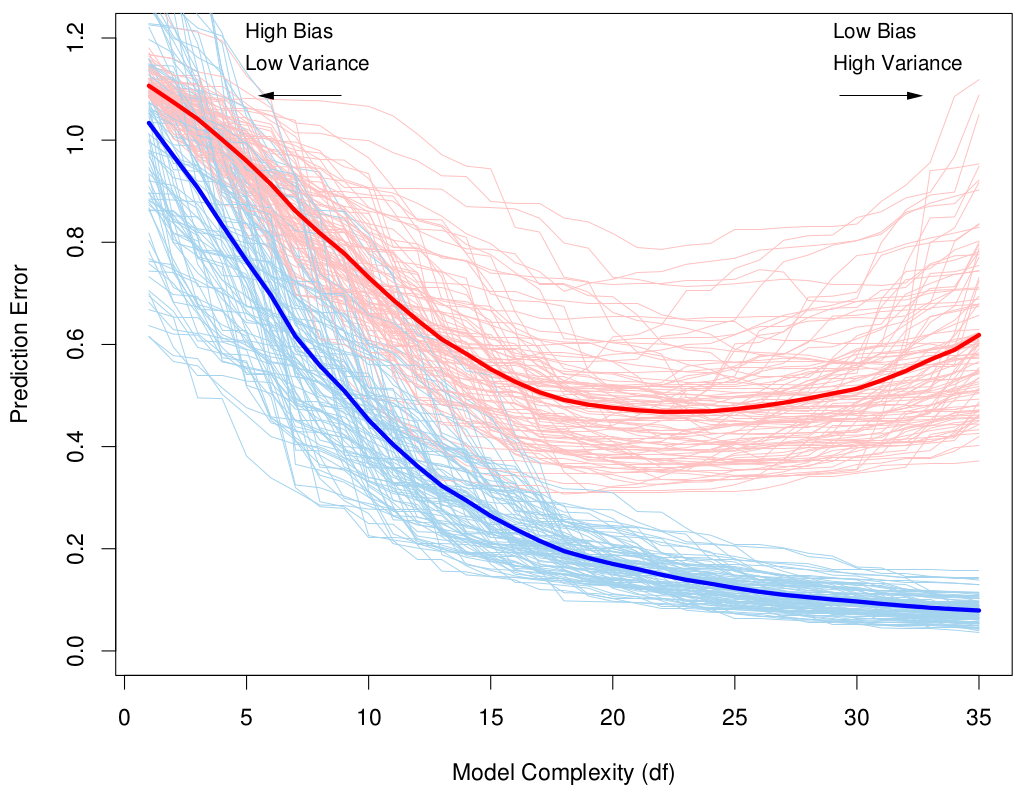
\includegraphics[width=0.89\textwidth]{biasVariance}
\end{figure}
}


\frame{\frametitle{Bias, Variance and Model Complexity: }
\framesubtitle{data split}
In an ideal (= a lot of data) situation, the best option is \textcolor{uio}{\bf randomly} \textcolor{uio}{splitting} the data in three \textcolor{uio}{\bf independent} sets,

\begin{center}
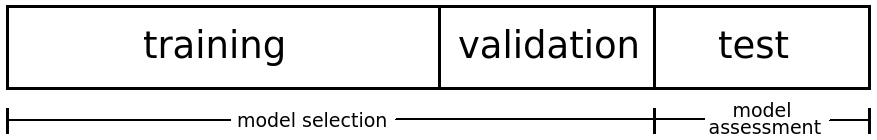
\includegraphics[width=0.89\textwidth]{dataSplit}
\end{center}

\begin{itemize}
\item {\bf training set:} data used to \textcolor{uio}{fit} the model(s);
\item {\bf validation set:} data used to \textcolor{uio}{identify} the best model;
\item {\bf test set:} data used to \textcolor{uio}{assess the performance} of the best model (must be completely ignored during model selection).
\end{itemize}
NB: it is extremely important to use the sets \textcolor{uio}{fully independently}!
}


\frame{\frametitle{Bias, Variance and Model Complexity: }
\framesubtitle{data split}

Example with k-nearest neighbour:
\begin{itemize}
\item in the {\bf training set:} \textcolor{uio}{fit} kNN with \textcolor{uio}{different values of $k$};
\item in the {\bf validation set:} \textcolor{uio}{select} the model with best performance (\textcolor{uio}{choose $k$});
\item in the {\bf test set:} \textcolor{uio}{evaluate} the prediction error of the model with the \textcolor{uio}{selected $k$}.
\end{itemize}
}


\frame{\frametitle{Bias, Variance and Model Complexity: }
\framesubtitle{data split}
How to \textcolor{uio}{split} the data in three set? There is not a general rule.

The book's suggestion:
\begin{itemize}
\item {\bf training set:} 50\%;
\item {\bf validation set:} 25\%;
\item {\bf test set:} 25\%.
\end{itemize}

\hspace{2pt}

We will see later what to do when there are no enough data;
\begin{itemize}
\item difficult to say when the data are ``enough''.
\end{itemize}
}


\subsection{The Bias--Variance Decomposition}

\frame{\frametitle{The Bias--Variance Decomposition: }
\framesubtitle{computations}
Consider $Y = f(X) + \epsilon$, $E[\epsilon]=0$, $\text{Var}[\epsilon]=\sigma^2$. Then
\begin{align*}
\text{Err}(x_0) &= E[(Y - \hat{f}(X))^2|X = x_0]\\ 
& = E[Y^2] + E[\hat{f}(x_0)^2] - 2E[Y\hat{f}(x_0))]\\
& = \text{Var}[Y] + f(x_0)^2 + \text{Var}[\hat{f}(x_0)] + E[\hat{f}(x_0)]^2 - 2 f(x_0) E[\hat{f}(x_0)]\\
& = \sigma^2 + \text{bias}^2(\hat{f}(x_0)) + \text{Var}[\hat{f}(x_0)]\\
& = \text{irreducible error} + \text{bias}^2 + \text{variance}
\end{align*} 
Remember that:
\begin{itemize}
\item $E[Y] = E[f(X)+\epsilon] = E[f(X)] + E[\epsilon] = f(X) + 0 = f(X)$;
\item $E[Y^2] = \text{Var}[Y] + E[Y]^2 = \sigma^2 + f(X)^2$;
\item $\hat{f}(X)$ and $\epsilon$ are uncorrelated.
\end{itemize}
}


\frame{\frametitle{The Bias--Variance Decomposition: }
\framesubtitle{k-nearest neighbours}
For the kNN regression:
\begin{align*}
\text{Err}(x_0) &= E_Y[(Y - \hat{f}_k(x_0))^2|X = x_0]\\
                &= \sigma^2_\epsilon + \left[f(x_0) - \frac{1}{k}\sum_{\ell=1}^k f(x_\ell)\right]^2 + \frac{\sigma_\epsilon^2}{k}
\end{align*}
Note:
\begin{itemize}
\item the number of neighbour is \textcolor{uio}{inversely related} to the complexity;
\item \textcolor{uio}{smaller $k$} $\rightarrow$ smaller bias, larger variance;
\item \textcolor{uio}{larger $k$} $\rightarrow$ larger bias, smaller variance.
\end{itemize}
}


\frame{\frametitle{The Bias--Variance Decomposition: }
\framesubtitle{linear regression}
For linear regression, with a \textcolor{uio}{$p$-dimensional} $\beta$ (regression coefficients) estimated by \textcolor{uio}{least squares},
\begin{align*}
\text{Err}(x_0) &= E_Y[(Y - \hat{f}_p(x_0))^2|X = x_0]\\
        &= \sigma^2_\epsilon + \left[f(x_0) - E[f_p(x_0)]\right]^2 + ||h(x_0)||^2\sigma_\epsilon^2
\end{align*}
where $h(x_0) = X(X^TX)^{-1}x_0$,
\begin{itemize}
\item $\hat{f}_p(x_0) = x_0^T(X^TX)^{-1}X^Ty$ $\rightarrow$ $\text{Var}[\hat{f}_p(x_0)] = ||h(x_0)||^2\sigma_\epsilon^2$.
\end{itemize}
In average,
$$
\frac{1}{N} \sum_{i = 1}^N \text{Err}(x_i) = \sigma^2_\epsilon + \frac{1}{N} \sum_{i = 1}^N \left[f(x_i) - E[f_p(x_i)]\right]^2 + \frac{p}{N}\sigma_\epsilon^2,
$$
so the model complexity is \textcolor{uio}{directly related} to $p$.
}


\frame{\frametitle{The Bias--Variance Decomposition: }
\framesubtitle{}
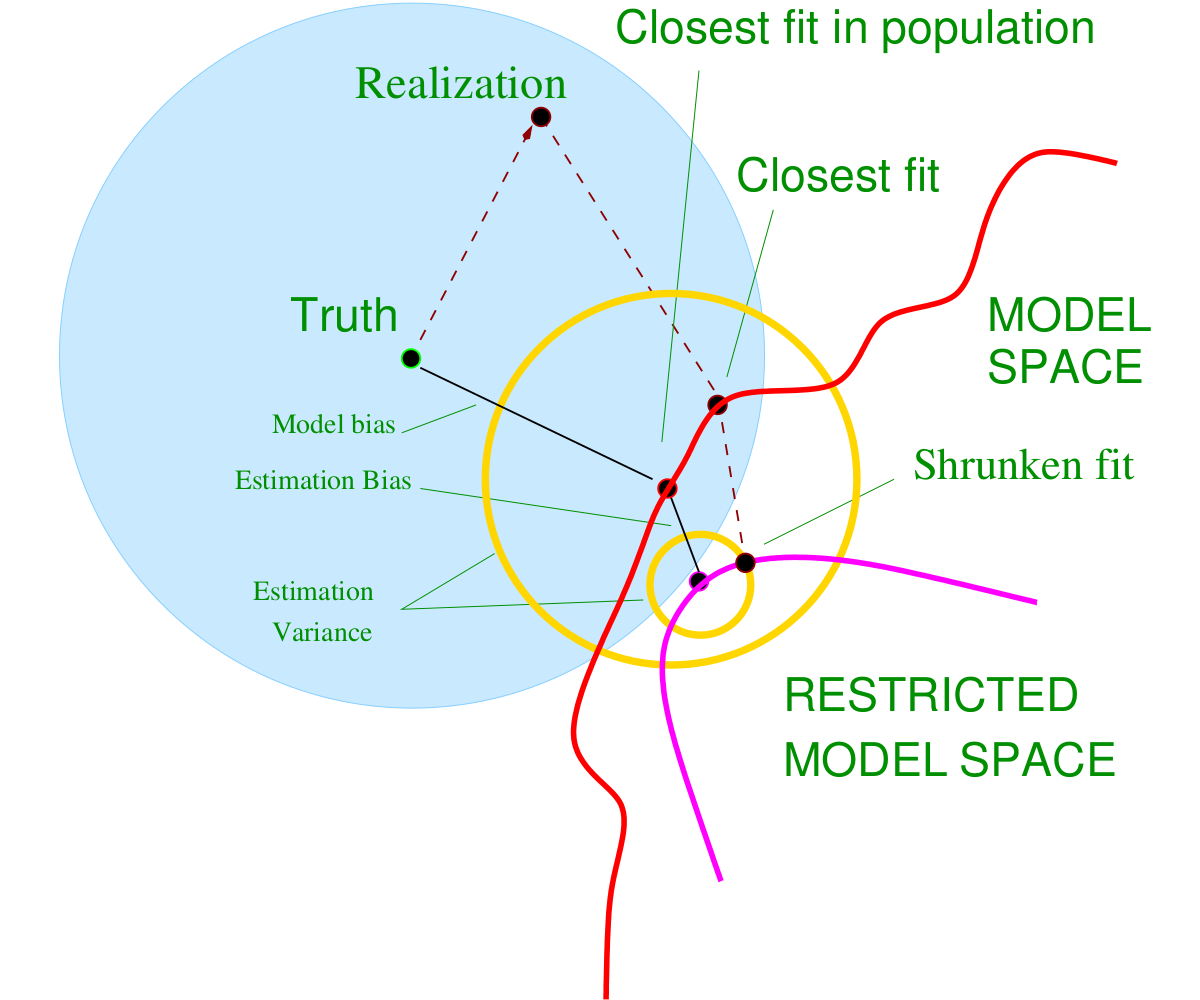
\includegraphics[width=\textwidth]{biasModel}
}

\frame{\frametitle{The Bias--Variance Decomposition: }
\framesubtitle{example}
\centering
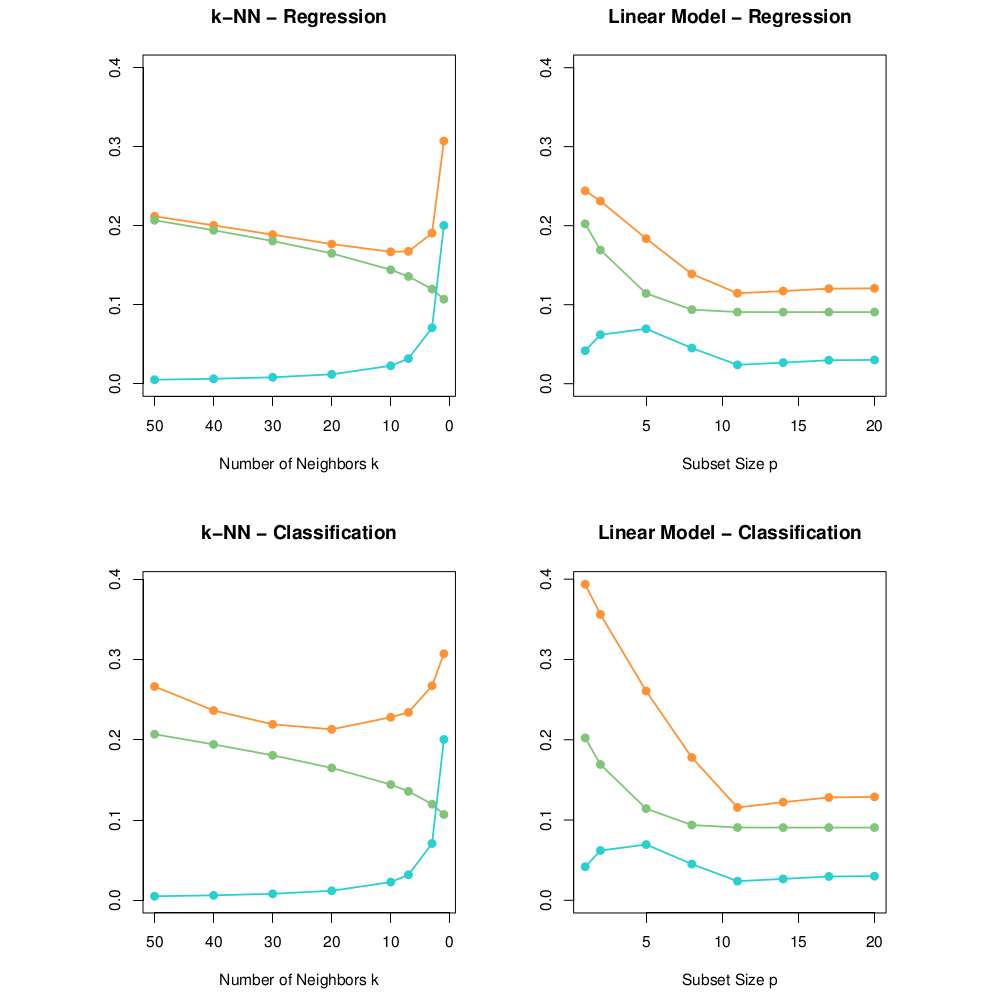
\includegraphics[width=0.71\textwidth]{diffLoss}
}




\subsection{Optimism of the Training Error Rate}

\frame{\frametitle{Optimism of the Training Error Rate: }
\framesubtitle{definitions}
Being a little bit more formal,
$$
\text{Err}_\mathcal{T} = E_{X_0,Y_0}[L(Y_0, \hat{f}(X_0))|\mathcal{T}]
$$
where:
\begin{itemize}
\item $(X_0, Y_0)$ are from the new test set;
\item $\mathcal{T} = \{(x_1,y_1)\dots (x_n,y_n)\}$ is fixed.
\end{itemize}

\hspace{2pt}

Taking the expected value over $\mathcal{T}$, we obtain the \textcolor{uio}{expected error}
$$
\text{Err} = E_\mathcal{T}\left[E_{X_0,Y_0}[L(Y_0, \hat{f}(X_0))|\mathcal{T}]\right].
$$
}

\frame{\frametitle{Optimism of the Training Error Rate: }
\framesubtitle{definitions}
We said that the \textcolor{uio}{training error},
$$
\widebar{\text{err}} = \frac{1}{N}\sum_{i = 1}^N L(y_i, \hat{f}(x_i)),
$$
is {\bf NOT} a good estimator of $\text{Err}_\mathcal{T}$:
\begin{itemize}
\item \textcolor{uio}{same data} used both for training and test;
\item a fitting method tends to \textcolor{uio}{adapt} to the specific dataset;
\item the result is a \textcolor{uio}{too optimistic evaluation of the error}.
\end{itemize}

\hspace{2pt}

How to measure this optimism?
}


\frame{\frametitle{Optimism of the Training Error Rate: }
\framesubtitle{optimism and average optimism}
Let us define the \textcolor{uio}{in-sample error},
$$
\text{Err}_\text{in} = \sum_{i = 1}^N E_{Y_0}[L(Y_{i0}, \hat{f}(x_i))|\mathcal{T}],
$$
i.e., the error computed w.r.t.\ new values of the outcome on the \textcolor{uio}{same} values of the \textcolor{uio}{training points} $x_i, i=1,\dots,N$.

\hspace{2pt}

We define \textcolor{uio}{optimism} the difference between $\text{Err}_\text{in}$ and $\widebar{\text{err}}$,
$$
\text{op} := \text{Err}_\text{in} - \widebar{\text{err}}.
$$
and the \textcolor{uio}{average optimism} its expectation,
$$
\omega := E_Y [\text{op}].
$$
NB: as the training points are fixed, the expected value is taken w.r.t. their outcomes.
}


\frame{\frametitle{Optimism of the Training Error Rate: }
\framesubtitle{optimism and average optimism}
For a reasonable number of \textcolor{uio}{loss functions}, including 0-1 loss and squared error, it can be shown that
$$
\omega = \frac{2}{N} \sum_{i = 1}^N \text{Cov}(\hat{y}_i,y_i),
$$
where:
\begin{itemize}
\item $\text{Cov}$ stands for covariance;
\item $\hat{y}_i$ is the prediction, $\hat{y}_i= \hat{f}(x_i)$;
\item $y_i$ is the actual value.
\end{itemize}

\hspace{2pt}

Therefore:
\begin{itemize}
\item optimism depends on \textcolor{uio}{how much $y_i$ affects its own prediction};
\item the \textcolor{uio}{``harder''} we fit the data, the \textcolor{uio}{larger} the value of $\text{Cov}(\hat{y}_i,y)$ $\rightarrow$ the \textcolor{uio}{larger} the optimism.
\end{itemize}
}

\frame{\frametitle{Optimism of the Training Error Rate: }
\framesubtitle{optimism and average optimism}
As a consequence,
$$
E_Y[\text{Err}_\text{in}] = E_Y[\widebar{\text{err}}] + \frac{2}{N}\sum_{i = 1}^N \text{Cov}(\hat{y}_i,y_i).
$$

\hspace{2pt}

When $\hat{y}_i$ is obtained by a linear fit of $d$ inputs the expression simplifies. For the linear additive model $Y=f(X)+\epsilon$,
$$
\sum_{i = 1}^N \text{Cov}(\hat{y}_i,y_i) = d \sigma^2_\epsilon,
$$
and
\begin{equation}\label{insample}
E_Y[\text{Err}_\text{in}] = E_Y[\widebar{\text{err}}] + 2\frac{d}{N}\sigma^2_\epsilon.
\end{equation}

Therefore:
\begin{itemize}
\item optimism \textcolor{uio}{increases linearly} with the number of predictors;
\item it \textcolor{uio}{decreases linearly} with the training sample size.
\end{itemize}
}


\frame{\frametitle{Optimism of the Training Error Rate: }
\framesubtitle{estimation}
Methods we will see:
\begin{itemize}
\item C$_p$, AIC, BIC \textcolor{uio}{estimate the optimism} and \textcolor{uio}{add} it to the \textcolor{uio}{training error} (work when estimates are linear in their parameters);
\item cross-validation and bootstrap directly estimate the \textcolor{uio}{expected error} (work in general).
\end{itemize}

\hspace{2pt}

Further notes:
\begin{itemize}
\item \textcolor{uio}{in-sample error} is in general \textcolor{uio}{NOT of interest};
\item when doing model selection/find the right model complexity, we are more interested in the \textcolor{uio}{relative difference in error} rather than the absolute one.
\end{itemize}
}



\subsection{Estimates of In-Sample Prediction Error}

\frame{\frametitle{Estimates of In-Sample Prediction Error: }
\framesubtitle{C$_p$}
Consider the general form of the in-sample estimates,
$$
\widehat{\text{Err}}_\text{in} = \widebar{\text{err}} + \hat{\omega}.
$$
Equation \eqref{insample},
$$ 
E_Y[\text{Err}_\text{in}] = E_Y[\widebar{\text{err}}] + 2\frac{d}{N}\sigma^2_\epsilon,
$$
in the case of linearity and square errors, leads to the \textcolor{uio}{C$_p$ statistics},
$$
\text{C}_p = \widebar{\text{err}} + 2\frac{d}{N}\hat{\sigma}^2_\epsilon,
$$
where:
\begin{itemize}
\item $\widebar{\text{err}}$ is the \textcolor{uio}{training error} computed by the square loss;
\item $d$ is the \textcolor{uio}{number of parameters} (e.g., regression coefficients);
\item $\hat{\sigma}^2_\epsilon$ is an estimate of the \textcolor{uio}{noise variance} (computed on the full model, i.e., that having the smallest bias).
\end{itemize}
}


\frame{\frametitle{Estimates of In-Sample Prediction Error: }
\framesubtitle{AIC}
Similar idea for \textcolor{uio}{AIC} (Akaike Information Criterion):
\begin{itemize}
\item we start from equation \eqref{insample};
\item more general by using a \textcolor{uio}{log-likelihood approach},
$$
-2E[\log p_{\hat{\theta}}(Y)] \approx -\frac{2}{N}E\left[\sum_{i=1}^N \log p_{\hat{\theta}}(y_i) \right] + 2 \frac{d}{N}
$$
Note that:
\begin{itemize}
\item the result holds \textcolor{uio}{asymptotically} (i.e., $N \rightarrow \infty$);
\item $p_{\hat{\theta}}(Y)$ is the \textcolor{uio}{family of densities} of $Y$, indexed by $\theta$;
\item $\sum_{i=1}^N \log p_{\hat{\theta}}(y_i) = \ell(\hat{\theta})$, the \textcolor{uio}{maximum likelihood estimate}.
\end{itemize}
\end{itemize}
Examples:
\begin{itemize}
\item logistic regression, $\text{AIC} = -\frac{2}{N}\ell(\hat{\theta}) + 2 \frac{d}{N}$;
\item linear regression, $\text{AIC} \; \propto \; \text{C}_p$.
\end{itemize}
}


\frame{\frametitle{Estimates of In-Sample Prediction Error: }
\framesubtitle{AIC}
To find the best model, we choose that with the \textcolor{uio}{smallest AIC}:
\begin{itemize}
\item straightforward in the simplest cases (e.g., linear models);
\item more attention must be devoted in more complex situations
\begin{itemize}
\item issue of finding a \textcolor{uio}{reasonable measure} for the \textcolor{uio}{model complexity};
\end{itemize}
\item[]
\end{itemize}
Usually \textcolor{uio}{minimizing the AIC} is \textcolor{uio}{not} the best solution to find the value of the \textcolor{uio}{tuning parameter}
\begin{itemize}
\item cross-validation works better in this case.
\end{itemize}
}


\subsection{The Effective Number of Parameters}

\frame{\frametitle{The Effective Number of Parameters}
\textcolor{uio}{Generalize} the concept of \textcolor{uio}{number of predictors} to extend the previous approaches to more complex situations.

Let
\begin{itemize}
\item $y = (y_1, \dots, y_n)$ be the outcome;
\item $\hat{y} = (\hat{y}_1, \dots, \hat{y}_n)$ be the prediction.
\item[]
\end{itemize}
For linear methods,
$$
\hat{y} = S y
$$
where $S$ is a $N \times N$ matrix which
\begin{itemize}
\item depend on $X$
\item does \textcolor{uio}{NOT depend} on $y$.
\end{itemize}
}


\frame{\frametitle{The Effective Number of Parameters}
The \textcolor{uio}{effective number of parameters} (or effective degrees of freedom) is defined as
$$
\text{df}(S) := \text{trace}(S);
$$
\begin{itemize}
\item $\text{trace}(S)$ is the \textcolor{uio}{sum of the diagonal elements} of $S$;
\item we should \textcolor{uio}{replace} $d$ with $\text{trace}(S)$ to obtain the correct value of the criteria seen before;
\item if $y=f(X)+\epsilon$, with $\text{Var}(\epsilon)=\sigma^2_\epsilon$, then $\sum_{i = 1}^N \text{Cov}(\hat{y}_i,y_i) = \text{trace}(S)\sigma^2_\epsilon$, which motivates
$$
\text{df}(\hat{y})= \frac{\sum_{i = 1}^N \text{Cov}(\hat{y}_i,y_i)}{\sigma^2_\epsilon}.
$$
\end{itemize}
}



\subsection{The Bayesian Approach and BIC}

\frame{\frametitle{The Bayesian Approach and BIC: }
\framesubtitle{BIC}
The \textcolor{uio}{BIC} (Bayesian Information Criterion) is an alternative criterion to AIC,
$$
\frac{1}{N}\text{BIC} = -\frac{2}{N} \ell(\hat{\theta}) + \log N \frac{d}{N}
$$
\begin{itemize}
\item similar to AIC, with \textcolor{uio}{$\log N$} instead of 2;
\item if $N > e^2 \approx 7.4$, BIC tends to favor \textcolor{uio}{simpler} models than AIC.
\item[]
\item For the Gaussian model,
$$
\text{BIC} = \frac{N}{\sigma^2_\epsilon}\left[\widebar{\text{err}} + (\log N) \frac{d}{N} \sigma^2_\epsilon\right].
$$

\end{itemize}
}


\frame{\frametitle{The Bayesian Approach and BIC: }
\framesubtitle{motivations}
Despite similarities, AIC and BIC come from \textcolor{uio}{different ideas}. In particular, BIC comes form the \textcolor{uio}{Bayesian model selection} approach.

Suppose
\begin{itemize}
\item $\mathcal{M}_m$, $m=1,\dots,M$ be a set of \textcolor{uio}{candidate models};
\item $\theta_m$ be their correspondent parameters;
\item $Z = {(x_1, y_1), \dots, (x_N, y_N)}$ be the training data.
\end{itemize}
Given the \textcolor{uio}{prior distribution} $Pr(\theta_m|\mathcal{M}_m)$ for all $\theta_m$, the posterior is
\begin{align*}
Pr(\mathcal{M}_m|z) & \propto Pr(\mathcal{M}_m) \cdot Pr(Z|\mathcal{M}_m)\\
  & \propto Pr(\mathcal{M}_m) \cdot \int_{\Theta_m} Pr(Z|\mathcal{M}_m, \theta_m) \cdot Pr(\theta_m|\mathcal{M}_m)\;d\theta_m.
\end{align*}
}


\frame{\frametitle{The Bayesian Approach and BIC: }
\framesubtitle{motivations}
To \textcolor{uio}{choose between} two models, we compare their posterior distributions,
$$
\frac{Pr(\mathcal{M}_m|z)}{Pr(\mathcal{M}_\ell|z)} = \underbrace{\frac{Pr(\mathcal{M}_m)}{Pr(\mathcal{M}_\ell)}}_\text{prior preference} \cdot \underbrace{\frac{Pr(Z|\mathcal{M}_m)}{Pr(Z|\mathcal{M}_\ell)}}_\text{Bayes factor}
$$
\begin{itemize}
\item usually the first term on the right hand side is \textcolor{uio}{equal to 1} (same prior probability for the two models);
\item the choice between the models is based on the \textcolor{uio}{Bayes factor}.
\end{itemize}
Using some algebra (including the Lapalce approximation), we find
$$
\log Pr(Z|\mathcal{M}_m) = \log Pr(Z|\hat{\theta}_m,\mathcal{M}_m)-\frac{d_m}{2}\log N + O(1).
$$
where:
\begin{itemize}
\item $\hat{\theta}_m$ is the maximum likelihood estimate of $\theta_m$;
\item $d_m$ is the number of free parameters in the model $\mathcal{M}_m$.
\end{itemize}

}


\frame{\frametitle{The Bayesian Approach and BIC: }
\framesubtitle{motivations}
Note:
\begin{itemize}
\item If the loss function is $-2\log Pr(Z|\hat{\theta}_m,\mathcal{M}_m)$, we find again the expression of \textcolor{uio}{BIC};
\item[]
\item selecting the model with \textcolor{uio}{smallest BIC corresponds} to selecting the model with the \textcolor{uio}{highest posterior} probability;
\item in particular, note that,
$$
\frac{e^{-\frac{1}{2}BIC_m}}{\sum_{\ell=1}^M e^{-\frac{1}{2}BIC_\ell}}
$$
is the \textcolor{uio}{probability of selecting} the model $m$ (out of $M$ models).
\end{itemize}
}


\frame{\frametitle{The Bayesian Approach and BIC: }
\framesubtitle{AIC versus BIC}
For \textcolor{uio}{model selection}, what to choose between AIC and BIC?
\begin{itemize}
\item there is \textcolor{uio}{no clear winner};
\item BIC leads to a \textcolor{uio}{sparser} model;
\item AIC tends to be better for \textcolor{uio}{prediction};
\item BIC is \textcolor{uio}{consistent} ($N\rightarrow \infty$, Pr(select the true model) $=1$);
\item for finite sample sizes, BIC tends to select a model which is \textcolor{uio}{too sparse}.
\end{itemize}
}


%%%%%%%%%%%%
%\section*{Bibliography}
%%%%%%%%%%%%
%
%\frame[allowframebreaks]{\frametitle{References}
%\footnotesize
%\bibliographystyle{../../../../support/biometrika}
%\bibliography{../../../../support/biblio}
%}

\end{document}
